% Editable source for rotation_counts.pdf (pdflatex rotation_counts.tex; pdftoppm -png -r 150 -singlefile rotation_counts.pdf rotation_counts).
% Exact, deterministic counts (no timing): canonical_rotation_steps of the frozen E-1 stage
% (8,000,000 target words, 4,000,000 index words), full scan and variant B from the frozen
% E-1 rows (run_1/run_2), lift_scan from this experiment's local exactness run (nonzero-shift
% candidate rotations; the lifting itself is 13 constant rotations per word, not counted here).
\documentclass[tikz,border=6pt]{standalone}
\usepackage[T1]{fontenc}
\usepackage{pgfplots}
\pgfplotsset{compat=1.17}
\begin{document}
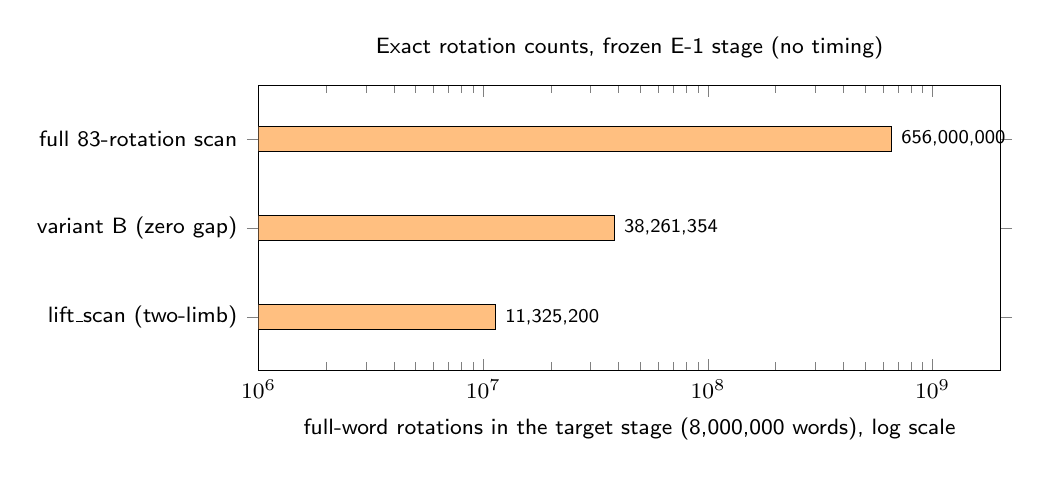
\begin{tikzpicture}[font=\sffamily\footnotesize]
\begin{axis}[xbar, width=11cm, height=5.2cm, xmode=log, log basis x=10,
  xmin=1e6, xmax=2e9, symbolic y coords={lift,gapB,full}, ytick=data,
  yticklabels={lift\_scan (two-limb), variant B (zero gap), full 83-rotation scan},
  xlabel={full-word rotations in the target stage (8,000,000 words), log scale},
  nodes near coords, nodes near coords style={font=\sffamily\scriptsize,anchor=west},
  point meta=explicit symbolic, bar width=9pt, enlarge y limits=0.3,
  title={Exact rotation counts, frozen E-1 stage (no timing)}]
\addplot[fill=orange!50] coordinates {(11325200,lift) [11,325,200] (38261354,gapB) [38,261,354] (656000000,full) [656,000,000]};
\end{axis}
\end{tikzpicture}
\end{document}
